
\documentclass{article}
\usepackage{afterpage}
\usepackage{float}
\usepackage{longtable}
\usepackage{graphicx}
\usepackage{pdflscape}
\usepackage[numbers,sort&compress]{natbib}
\usepackage{psfrag}

\usepackage{amsmath}
\usepackage{amsfonts}
\usepackage{graphicx}
%\usepackage{nicefrac}
\usepackage{graphicx}
\usepackage{caption}
% \usepackage{subcaption}
\usepackage{subfigure}
% \usepackage{algorithm}
% \usepackage{paralist}
% % \usepackage[geometry]{ifsym}
\usepackage{rotating}
\usepackage{setspace}
\newcommand{\uu}[1]{\boldsymbol #1}
\usepackage{listings}
\usepackage{xcolor}
\usepackage{subfigure}
\usepackage{fullpage}
\lstset{language=C++,
                keywordstyle=\color{blue},
                stringstyle=\color{red},
                commentstyle=\color{green},
                morecomment=[l][\color{magenta}]{\#}
}
\doublespace
\begin{document}


\section*{Exact solutions}

Pure dirichlet boundary conditions with analytical solution:
\begin{align*} \nonumber
&\uu{u}(x,y)= \begin{pmatrix}
  xy\exp(x + y) + x\exp(x + y)\\
  -xy\exp(x + y) - y\exp(x + y)
\end{pmatrix}, \\
&p(x,y) = \exp(y)\sin(x),\\
&\uu{b}(x,y) = \begin{pmatrix}
 \exp(x + y)\cos(x) \\
 \exp(x + y)\sin(x) - \exp(x + y)\cos(x)
\end{pmatrix}, \\
 &r(x,y) = x\sin(2\pi x)\sin(2\pi y).
\end{align*}



\begin{figure}[h!]
    \centering
    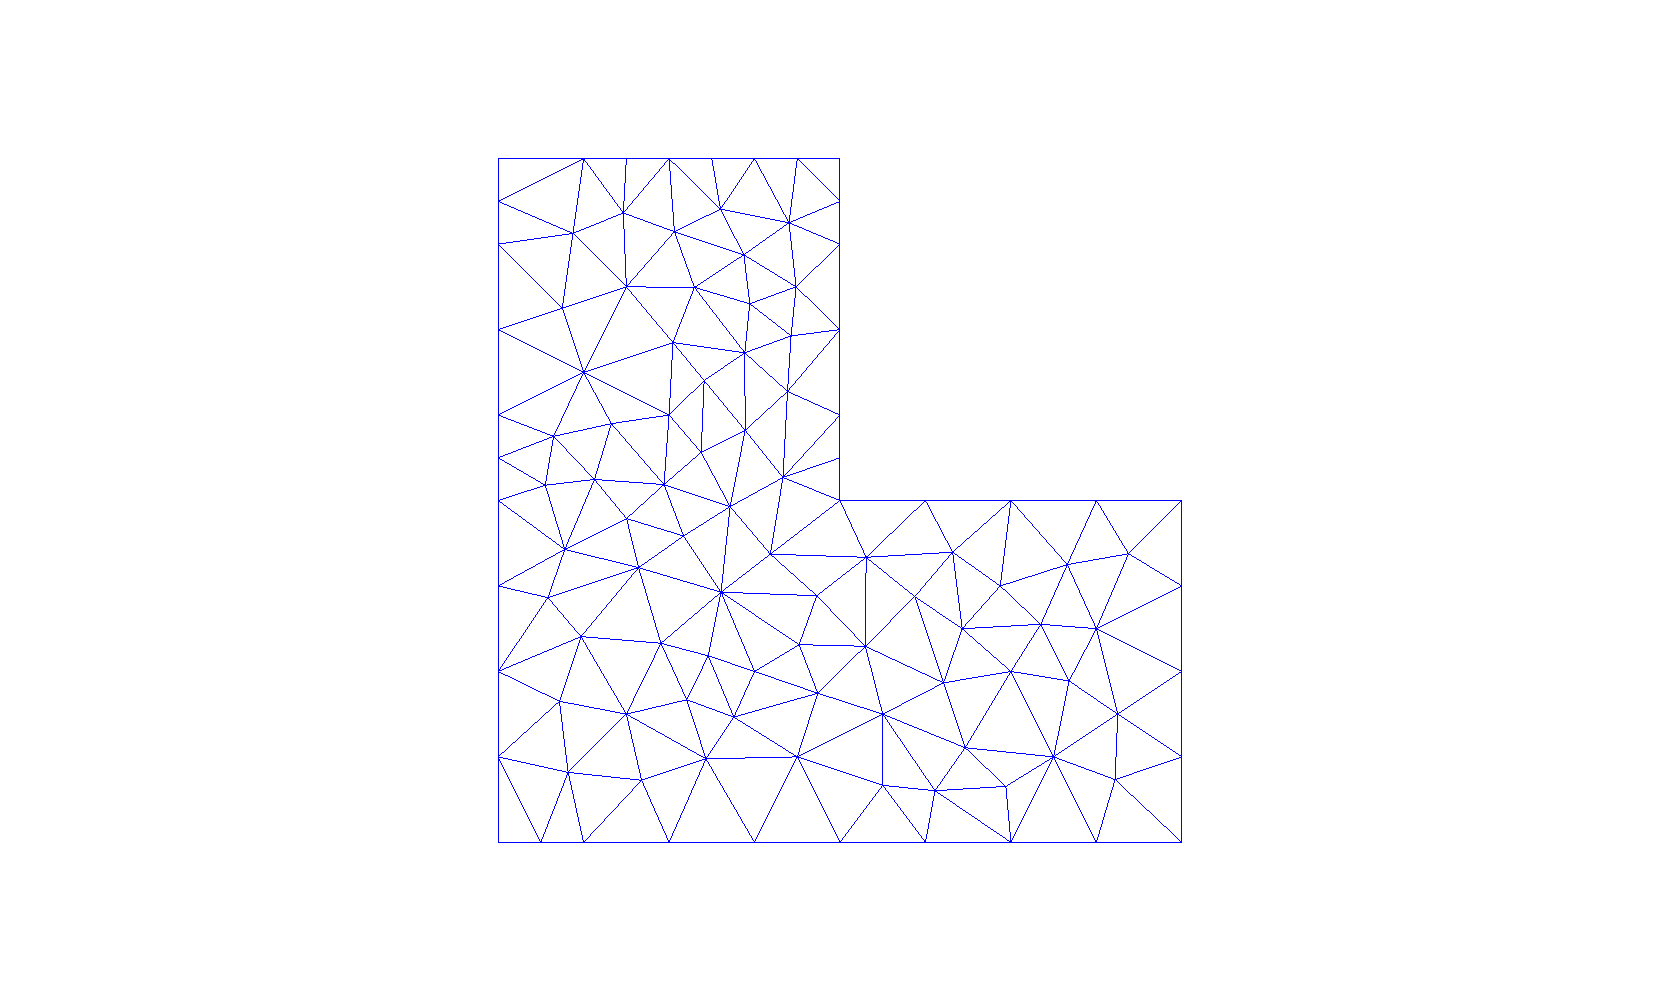
\includegraphics[width=0.6\textwidth]{../Lshaped.png}
    \caption{Lshaped domain}
    \label{fig:awesome_image}
\end{figure}
\section*{Preconditioner results - direct application of preconditioners}

\begin{table}[h!]
\centering
\begin{tabular}{ccccccccccc}
\hline
$\ell$ & DoF &  time$_{\rm solve}$ &  time$_{\rm NL}$ &  it$_{\rm NL}$ & it$_{\rm av}$ \\
\hline
1 &      71 & 0.00 & 0.29 & 15 & 22.0 \\
2 &     242 & 0.02 & 0.56 & 16 & 81.1 \\
3 &     909 & 0.03 & 1.34 & 24 & 59.8 \\
4 &    3,283 & 0.08 & 4.14 & 29 & 52.2 \\
5 &   12,867 & 0.35 & 16.91 & 30 & 52.1 \\
6 &   51,379 & 1.87 & 85.92 & 31 & 52.8 \\
7 &  203,556 & 12.37 & 504.08 & 31 & 53.8 \\
\hline
\end{tabular}
\end{table}

\newpage

\section*{Convergence results - direct solves on linear system}

\begin{table}[h!]
\begin{center}
\begin{tabular}{cccccccccc}
\hline
$\ell$ &    Dofs $\uu{u}_h/p_h$ & $\|\uu{u}-\uu{u}_h\|_{L^2(\Omega)}$ & order & $\|\uu{u}-\uu{u}_h\|_{H^1(\Omega)}$ & order  &  $\|{p}-{p}_h\|_{L^2(\Omega)}$ & order \\
\hline
 1 & 42/8 &  8.8613e+00 &     0.00 &  5.5371e+01 &     0.00 &  4.5613e+02 &      0.00 \\
 2 & 146/23 &  4.1281e+00 &     1.10 &  4.5019e+01 &     0.30 &  1.0459e+02 &      2.12 \\
 3 & 554/78 &  6.5366e-01 &     2.66 &  1.2378e+01 &     1.86 &  2.7443e+01 &      1.93 \\
 4 & 2,010/268 &  1.1755e-01 &     2.48 &  2.9325e+00 &     2.08 &  4.6939e+00 &      2.55 \\
 5 & 7,898/1,020 &  2.5188e-02 &     2.22 &  8.7477e-01 &     1.75 &  1.1816e+00 &      1.99 \\
 6 & 31,578/4,012 &  6.3267e-03 &     1.99 &  2.7412e-01 &     1.67 &  3.3121e-01 &      1.83 \\
 7 & 125,186/15,777 &  1.4864e-03 &     2.09 &  7.4636e-02 &     1.88 &  7.6414e-02 &      2.12 \\
\hline
\end{tabular}
\caption{Convergence of velocity/pressure field}
\label{tab:NS_2D_smooth_velocity}
\end{center}
\end{table}


\begin{table}[h!]
\begin{center}
\begin{tabular}{cccccc}
\hline
$\ell$ &    Dofs $\uu{b}_h/r_h$ & $\|\uu{b}-\uu{b}_h\|_{L^2(\Omega)}$ & order & $\|\uu{b}-\uu{b}_h\|_{H({\rm curl},\Omega)}$ & order \\
\hline
1 &     13/8 &  9.8687e+00 &     0.00 &  1.2202e+01 &        0.00 \\
2 &     50/23 &  4.6256e+00 &     1.09 &  8.8619e+00 &        0.46 \\
3 &    199/78 &  1.8629e+00 &     1.31 &  4.6257e+00 &        0.94 \\
4 &    737/268 &  8.7549e-01 &     1.09 &  2.1267e+00 &        1.12 \\
5 &   2,929/1,020 &  4.2624e-01 &     1.04 &  1.0126e+00 &        1.07 \\
6 &  11,777/4,012 &  2.1315e-01 &     1.00 &  5.4336e-01 &        0.90 \\
7 &  46,816/15,777 &  1.0649e-01 &     1.00 &  2.6991e-01 &        1.01 \\
\hline
\end{tabular}
\caption{Convergence for magnetic field}
\label{tab:2D_maxwell_magnetic}
\end{center}
\end{table}
\begin{table}[h!]
\begin{center}
\begin{tabular}{cccccc}
\hline
$\ell$ &    Dofs $\uu{b}_h/r_h$ & $\|{r}-{r}_h\|_{L^2(\Omega)}$ & order & $\|{r}-{r}_h\|_{H^1(\Omega)}$ & order\\
\hline
 1 &      13/8 &     9.7025e-01 &     0.00 &  1.0103e+01 &     0.00 \\
 2 &     50/23 &     1.5270e+00 &     0.65 &  1.2310e+01 &     0.29 \\
 3 &     199/78 &     4.3060e-01 &     1.83 &  5.0480e+00 &     1.29 \\
 4 &    737/268 &     8.5258e-02 &     2.34 &  2.3952e+00 &     1.08 \\
 5 &   2,929/1,020 &    2.2436e-02 &     1.93 &  1.1695e+00 &     1.03 \\
 6 &   11,777/4,012 &    5.4642e-03 &     2.04 &  5.7658e-01 &     1.02 \\
 7 &  46,816/15,777 &  1.3809e-03 &     1.98 &  2.9065e-01 &     0.99 \\

\hline
\end{tabular}
\caption{Convergence for  multiplier variable}
\label{tab:2D_maxwell_multiplier}

\end{center}
\end{table}



\end{document}
